\let\negmedspace\undefined
\let\negthickspace\undefined
\documentclass[journal,12pt,twocolumn]{IEEEtran}
\usepackage{float}
\usepackage{circuitikz}
\usepackage{cite}
\usepackage{amsmath,amssymb,amsfonts,amsthm}
\usepackage{algorithmic}
\usepackage{graphicx}
\usepackage{textcomp}
\usepackage{xcolor}
\usepackage{txfonts}
\usepackage{listings}
\usepackage{amsmath}
\usepackage{enumitem}
\usepackage{mathtools}
\usepackage{gensymb}
\usepackage{comment}
\usepackage[breaklinks=true]{hyperref}
\usepackage{tkz-euclide} 
\usepackage{listings}
\usepackage{gvv}                                        
\def\inputGnumericTable{}                                 
\usepackage[latin1]{inputenc}                                
\usepackage{color}                                            
\usepackage{array}                                            
\usepackage{longtable}                                       
\usepackage{calc}                                             
\usepackage{multirow}                                         
\usepackage{hhline}                                           
\usepackage{ifthen}                                           
\usepackage{lscape}
\newtheorem{theorem}{Theorem}[section]
\newtheorem{problem}{Problem}
\newtheorem{proposition}{Proposition}[section]
\newtheorem{lemma}{Lemma}[section]
\newtheorem{corollary}[theorem]{Corollary}
\newtheorem{example}{Example}[section]
\newtheorem{definition}[problem]{Definition}
\newcommand{\BEQA}{\begin{eqnarray}}
\newcommand{\EEQA}{\end{eqnarray}}
\newcommand{\define}{\stackrel{\triangle}{=}}
\theoremstyle{remark}
\newtheorem{rem}{Remark}
\begin{document}

\bibliographystyle{IEEEtran}
\title{ AUDIO FILTERING ASSIGNMENT}
\author{EE23BTECH11011- Batchu Ishitha$^{*}$% <-this % stops a space
}
\maketitle

\bigskip

\renewcommand{\thefigure}{\theenumi}
\renewcommand{\thetable}{\theenumi}
%\renewcommand{\theequation}{\theenumi}

\section{DIGITAL FILTER}
\begin{enumerate}[label=\thesection\arabic*.,ref=\thesection.\theenumi]
\item The sound file used for this code can be obtained from the following link.
\begin{lstlisting}

\end{lstlisting}

\item Python code for removal of out of band noise:
\lstinputlisting{./codes/1.2.py} 
\item Analysis of sound file before and after removal of noise using spectrogram ie: https://academo.org/demos/spectrum-analyzer.
\begin{figure}[ht]
    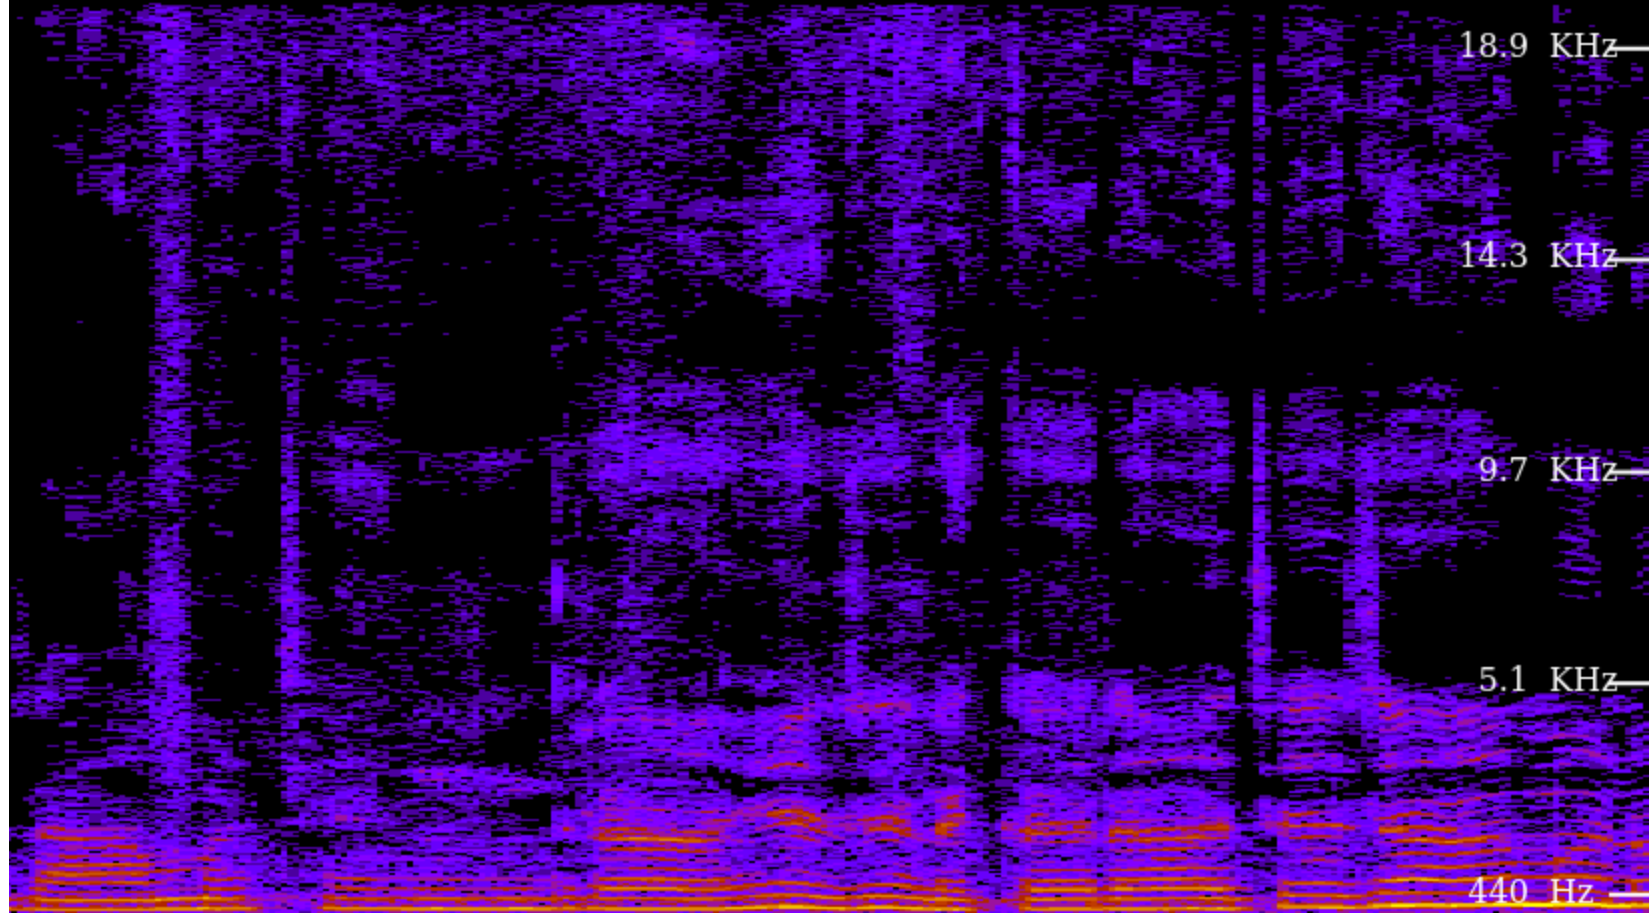
\includegraphics[width=0.8\columnwidth]{figs/beforefiltering.png }
    \caption{Spectrogram of the audio file before Filtering}
    \label{fig:beforefiltering}
\end{figure}
\begin{figure}[ht]
    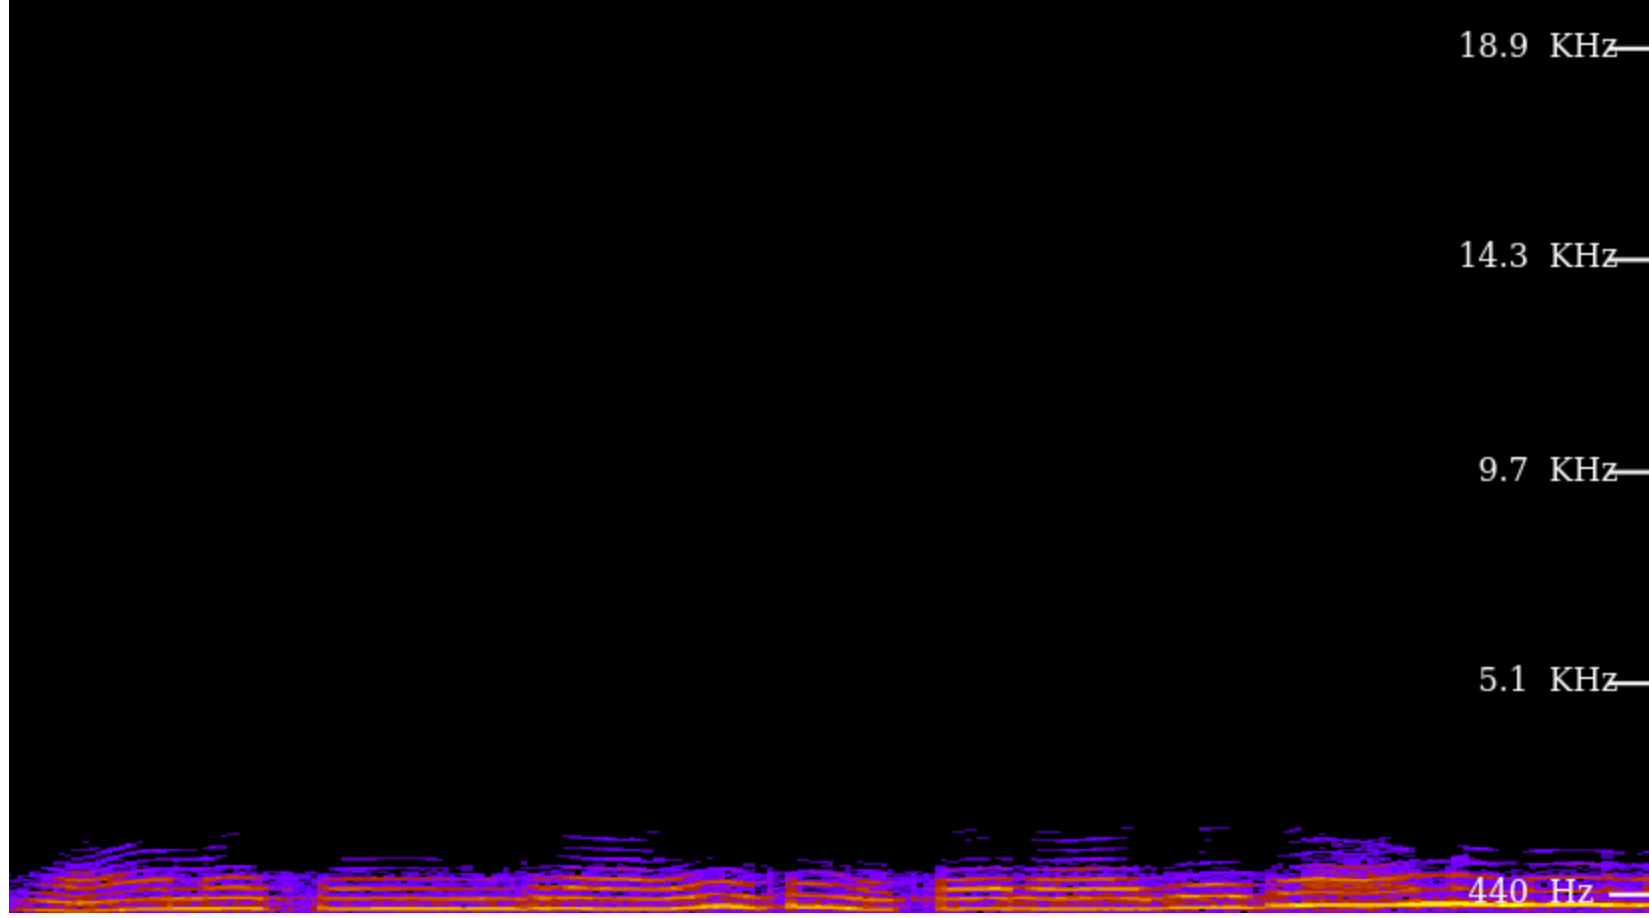
\includegraphics[width=0.8\columnwidth]{figs/afterfiltering.png}
    \caption{Spectrogram of the audio file after Filtering}
    \label{fig:afterfiltering}
\end{figure}
\end{enumerate}

\section{DIFFERENCE EQUATION}
\begin{enumerate}[label=\thesection\arabic*.,ref=\thesection.\theenumi]
\item Let
\begin{align}
x(n) &= \cbrak{\underset{\uparrow}{1},2,3,4,2,1}
\end{align}
Sketch $x(n)$.
\item Let 
\begin{align}
y(n) +\frac{1}{2}y(n-1) &= x(n) + x(n-2),\nonumber \\ 
& \hspace{2cm} y(n)=0, n<0
\end{align}
\end{enumerate}
\solution  C code for generating values of y(n):
\begin{lstlisting}
\end{lstlisting} 
Python code for plotting x(n) and y(n):
\begin{lstlisting}
\end{lstlisting}
\begin{figure}[ht]
	\centering
	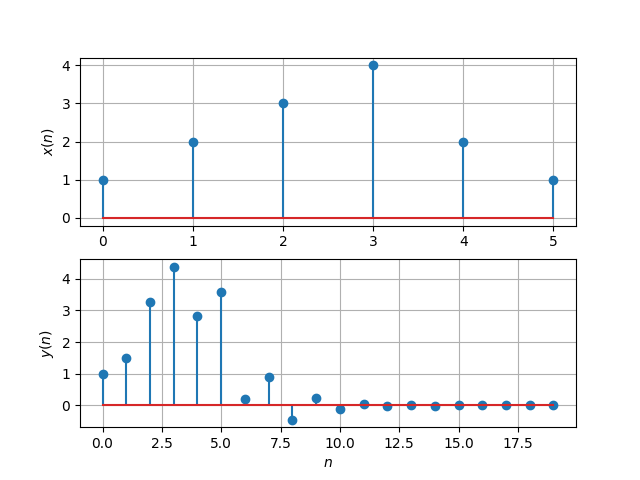
\includegraphics[width=\columnwidth]{figs/xnyn}
	\caption{Plot of $x(n)$ and $y(n)$}
	\label{fig:xnyn}
\end{figure}


\end{document}
